\chapter{Accurate Newton's Method for B\'{e}zier Curve Intersection}
\label{chap:compensated-newton}

\section{Introduction}

When using Newton's method to find the root of a function via
\begin{equation}
G\left(\bm{x}\right) = \bm{x} - J^{-1} F\left(\bm{x}\right)
\end{equation}
there are three computations performed that can introduce instability:
evaluation of the residual function \(F\left(\bm{x}\right)\), evaluation
of the Jacobian \(J\) and solution of the linear system \(J \bm{y} =
F\left(\bm{x}\right)\). In \cite{Tisseur2001}, the author showed that by
just using a more precise evaluation of the residual function, the
accuracy of Newton's method can be improved.

This chapter considers Newton's method applied to two problems:
root-finding for polynomials expressed in Bernstein form and
intersection of two B\'{e}zier curves in \(\reals^2\). In both problems,
the compensated de Casteljau method (see Chapter~\ref{chap:k-compensated}) is
used for evaluation of the residual. When evaluating a polynomial
\(p(s)\) this is straightforward, but when evaluating the difference
\(b_1(s) - b_2(t)\) between two curves special care must be taken.

\begin{figure}
  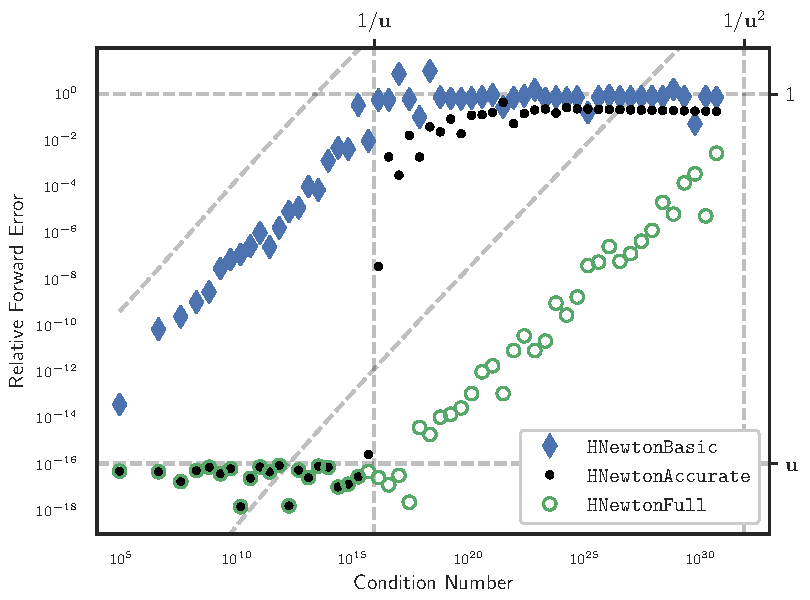
\includegraphics{../images/compensated-newton/newton_jghplus13.pdf}
  \centering
  \captionsetup{width=.75\linewidth}
  \caption{Comparing relative error to condition number when using Newton's
    method to find a root of \(p(x) = (x - 1)^n - 2^{-31}\), where polynomial
    evaluation occurs via Horner's method.}
  \label{fig:jgh+13}
\end{figure}

In \cite{Graillat2008}, the problem of finding simple polynomial roots for
polynomials expressed in the monomial basis is considered. There the author
showed that using a compensated Horner's method to evaluate the residual
(\texttt{NewtonAccurate}) approximates roots with \(\bigO{\mach}\) relative
error. This gain in accuracy holds until the condition number of evaluation
reaches \(1/\mach\), at which point the relative error jumps to \(\bigO{1}\)
as can be seen in Figure~\ref{fig:jgh+13}. This abrupt change in error is not
unexpected given what is shown in \cite{Tisseur2001}, though it starkly
differs from the way the error gradually increases with the condition
number with standard non-compensated Newton's method (\texttt{NewtonBasic}).
In \cite[Section~8]{Jiang2013}, the author follows up by showing that a
compensated evaluation of the Jacobian\footnote{In the one dimensional case,
it's just the derivative of the polynomial.} (\texttt{NewtonFull}) enables
such a gradual descrease in error as the condition number grows from
\(1/\mach\) to \(1/\mach^2\). We'll proceed similarly for polynomials in
Bernstein form. Since this is a one dimensional Newton's method, improving
the evaluation of the Jacobian is straightforward. The results agree with
what has been observed when using Horner's method for evaluation.

Computing the intersection(s) of two parametric plane curves is a
common task in computational geometry and has many uses, e.g. in
finite element methods that use overlapping curved meshes. Many
methods have been described in the literature to solve this problem.
Algebraic methods such as implicitization and eigenvalue-based
methods (e.g. \cite{Manocha:CSD-92-698}) suffer
from accuracy issues for moderately high degrees and can often be
very complex to implement. Some (\cite{Bates2008}) even rely on symbolic
algebraic manipulations, which can be quite costly since it requires
arbitrary precision.
Geometric methods (e.g. \cite{Sederberg1986, Sederberg1990, Kim1998})
typically use a form of domain splitting to focus on subproblems and
eliminate parts of the domain where an intersection is guaranteed not
to occur. After a domain has been sufficiently reduced, Newton's method
is used for the last few bits of accuracy.

We'll focus on transversal curve intersections that are ill-conditioned.
Transversal intersections are an extension of the concept of a
simple root. A non-transversal intersection occurs when the curves
or tangent at the point of intersection or when one of the curves
has a zero tangent vector at that point, either due to an improper
parameterization (e.g. \(x(s) = s^2, y(s) = s^2 + 1\)) or a cusp.
In many cases, transversal intersections that are ``almost tangent'' have
very high condition numbers.

The chapter is organized as follows. In Section~\ref{sec:conditioning}
we define and discuss the conditioning of both a simple root and
a transversal intersection. In Section~\ref{sec:compensated-numerical}
we perform two numerical experiments to give practical examples of the
theoretical error bounds. Section~\ref{sec:false-starts} acts as a
coda: it describes some failed attempts at constructing numerical
examples. This section provides an in-depth discussion of a particular
family of polynomials that has much better than expected conditioning
when written in the Bernstein basis.

\section{Problem conditioning}\label{sec:conditioning}

Placeholder.

\section{Numerical experiments}\label{sec:compensated-numerical}

Placeholder.

\section{False starts}\label{sec:false-starts}

Placeholder.
